% Section: Reference controller
\section{Reference controller}
\label{sec:reference}

\subsection{Controller}
\label{subsec:discon}
{\color{revQ1}
The reference controller is the baseline controller of the NREL 5-MW turbine~\cite{jonkman2009}: a variable-speed generator-torque law over control regions 1 to 3, and a gain-scheduled proportional-integral collective-pitch controller acting on the filtered generator speed, with pitch-angle and pitch-rate limits. Its source file DISCON.F90, taken from the OpenFAST regression-test suite, was compiled here with GNU Fortran 8.1.0 into a dynamic library, without any change to its gains or constants. The library was accepted after the means of rotor speed, blade pitch angle, generator torque and generator power over the regression-test case of the land-based turbine with this controller agreed with the reference outputs of that case within the acceptance tolerance of the test. The reference outputs of the regression test were produced with another build of OpenFAST and of the controller, whose compiler is not documented for this file.
}

\subsection{Coupling with OpenFAST}
\label{subsec:coupling}
{\color{revQ1}
All the controllers compared in this paper, the reference controller and the NMPC arms, drive the same plant: OpenFAST v4.2.1 run as a Simulink S-function, which receives the collective pitch command and the generator torque at every time step of 0.00625~s. The reference controller is called at every time step through a MATLAB wrapper of the compiled library. Fed with the inputs recorded in a run of the standalone OpenFAST executable, this wrapper reproduced the pitch and torque commands of that run within a tolerance fixed before the test. In closed loop, the wrapper passes the measured blade pitch angle to the controller, and OpenFAST runs with the interpolation order of the model (InterpOrder = 2) and one correction iteration per time step (NumCrctn = 1), whereas the corresponding regression-test case uses none (NumCrctn = 0). This setting was retained, by a comparison with the standalone executable defined before it was run, after the pitch loop had diverged with other settings of the coupling; why the pitch loop did not diverge with this setting is not explained here. Figure~\ref{fig:E3_loop} illustrates this closed loop and the main signals exchanged at every time step.

Two limits of this coupling are declared. First, the plant-equivalence test, in which the commands recorded with the standalone executable were replayed through the S-function, was not concordant at the tolerance fixed before the test: the maximum deviation of the blade pitch angle, which follows the replayed command, exceeded the tolerance, while the rotor speed, the generator power and the tower-base and blade-root bending moments were within it. The S-function plant is therefore used for every controller, and its results are never mixed with runs of the standalone executable. Second, at initialization the S-function receives a zero generator torque before the first controller call, which causes a start-up transient that was not quantified.
}

\begin{figure}[htbp]
\centering
% Figure E3-1 of Paper_Q1 (section 3.2): closed loop of configuration O8. Schematic only: no data and
% no result number (openfast_q1/docs/spec_figures_E3_E4.yaml, E3_1_loop and general.schematics).
% Content as coded in openfast_q1/E3/run_E3b.m and openfast_q1/E4/run_E4.m: FAST_SFunc outputs go to
% the MATLAB Function block, which calls discon_wrapper and DISCON.dll at every DT = 0.00625 s; the
% measured BldPitch1 and GenSpeed go to DISCON; generator torque (input 1), electrical power (input 2)
% and collective pitch command (inputs 5-7) go back to FAST_SFunc; the dashed frame marks where the
% NMPC arms replace DISCON at Ts = 0.05 s (spec_E2 nmpc_interface.Ts.main).
% Requires \usepackage{tikz}, \usetikzlibrary{arrows.meta, positioning, calc} and siunitx
% (Paper_Q1/main.tex). Included with % Figure E3-1 of Paper_Q1 (section 3.2): closed loop of configuration O8. Schematic only: no data and
% no result number (openfast_q1/docs/spec_figures_E3_E4.yaml, E3_1_loop and general.schematics).
% Content as coded in openfast_q1/E3/run_E3b.m and openfast_q1/E4/run_E4.m: FAST_SFunc outputs go to
% the MATLAB Function block, which calls discon_wrapper and DISCON.dll at every DT = 0.00625 s; the
% measured BldPitch1 and GenSpeed go to DISCON; generator torque (input 1), electrical power (input 2)
% and collective pitch command (inputs 5-7) go back to FAST_SFunc; the dashed frame marks where the
% NMPC arms replace DISCON at Ts = 0.05 s (spec_E2 nmpc_interface.Ts.main).
% Requires \usepackage{tikz}, \usetikzlibrary{arrows.meta, positioning, calc} and siunitx
% (Paper_Q1/main.tex). Included with % Figure E3-1 of Paper_Q1 (section 3.2): closed loop of configuration O8. Schematic only: no data and
% no result number (openfast_q1/docs/spec_figures_E3_E4.yaml, E3_1_loop and general.schematics).
% Content as coded in openfast_q1/E3/run_E3b.m and openfast_q1/E4/run_E4.m: FAST_SFunc outputs go to
% the MATLAB Function block, which calls discon_wrapper and DISCON.dll at every DT = 0.00625 s; the
% measured BldPitch1 and GenSpeed go to DISCON; generator torque (input 1), electrical power (input 2)
% and collective pitch command (inputs 5-7) go back to FAST_SFunc; the dashed frame marks where the
% NMPC arms replace DISCON at Ts = 0.05 s (spec_E2 nmpc_interface.Ts.main).
% Requires \usepackage{tikz}, \usetikzlibrary{arrows.meta, positioning, calc} and siunitx
% (Paper_Q1/main.tex). Included with \input{figures/E3_fig1_loop} inside a figure environment of
% section 3 (step 5 of spec_figures_E3_E4 order).
\begin{tikzpicture}[
    >={Stealth[length=2.2mm]},
    blk/.style={draw, thick, align=center, font=\small, inner sep=2mm},
    sig/.style={font=\footnotesize, align=center}
  ]
  % plant
  \node[blk, minimum width=32mm, minimum height=26mm] (fast) at (0, 0)
    {\texttt{FAST\_SFunc}\\[2pt]{\footnotesize OpenFAST plant}\\{\footnotesize PCMode 4, VSContrl 4}};
  % baseline controller, called by the MATLAB Function block
  \node[blk, minimum width=34mm, minimum height=9mm] (wrap) at (9.6, 0.85) {\texttt{discon\_wrapper}};
  \node[blk, minimum width=34mm, minimum height=9mm] (dll)  at (9.6, -0.85) {\texttt{DISCON.dll}};
  \draw[<->] (wrap) -- (dll);
  % dashed frame: part replaced by the NMPC arms
  \draw[dashed, thick] ($(wrap.north west) + (-2.5mm, 2.5mm)$) rectangle ($(dll.south east) + (2.5mm, -2.5mm)$);
  % MATLAB Function block
  \coordinate (mnw) at ($(wrap.north west) + (-6mm, 8mm)$);
  \coordinate (mse) at ($(dll.south east) + (6mm, -8mm)$);
  \draw[thick] (mnw) rectangle (mse);
  \node[sig, align=left, anchor=south west] at (mnw)
    {MATLAB Function block,\\called every $\mathrm{DT} = 0.00625\,\mathrm{s}$};
  % signals between the plant and the block
  \coordinate (inA) at (mnw |- fast.east);
  \draw[->, thick] ($(fast.east) + (0, 6mm)$) --
    node[sig, above] {measured \texttt{BldPitch1}\\and \texttt{GenSpeed} to DISCON}
    ($(inA) + (0, 6mm)$);
  \draw[->, thick] ($(inA) + (0, -6mm)$) --
    node[sig, below] {generator torque (input 1)\\electrical power (input 2)\\collective pitch command\\(inputs 5--7)}
    ($(fast.east) + (0, -6mm)$);
  % meaning of the dashed frame
  \node[sig, align=right, anchor=north east] at (mse)
    {dashed frame: replaced by the\\NMPC arms at $T_s = \SI{0.05}{\second}$};
\end{tikzpicture}
 inside a figure environment of
% section 3 (step 5 of spec_figures_E3_E4 order).
\begin{tikzpicture}[
    >={Stealth[length=2.2mm]},
    blk/.style={draw, thick, align=center, font=\small, inner sep=2mm},
    sig/.style={font=\footnotesize, align=center}
  ]
  % plant
  \node[blk, minimum width=32mm, minimum height=26mm] (fast) at (0, 0)
    {\texttt{FAST\_SFunc}\\[2pt]{\footnotesize OpenFAST plant}\\{\footnotesize PCMode 4, VSContrl 4}};
  % baseline controller, called by the MATLAB Function block
  \node[blk, minimum width=34mm, minimum height=9mm] (wrap) at (9.6, 0.85) {\texttt{discon\_wrapper}};
  \node[blk, minimum width=34mm, minimum height=9mm] (dll)  at (9.6, -0.85) {\texttt{DISCON.dll}};
  \draw[<->] (wrap) -- (dll);
  % dashed frame: part replaced by the NMPC arms
  \draw[dashed, thick] ($(wrap.north west) + (-2.5mm, 2.5mm)$) rectangle ($(dll.south east) + (2.5mm, -2.5mm)$);
  % MATLAB Function block
  \coordinate (mnw) at ($(wrap.north west) + (-6mm, 8mm)$);
  \coordinate (mse) at ($(dll.south east) + (6mm, -8mm)$);
  \draw[thick] (mnw) rectangle (mse);
  \node[sig, align=left, anchor=south west] at (mnw)
    {MATLAB Function block,\\called every $\mathrm{DT} = 0.00625\,\mathrm{s}$};
  % signals between the plant and the block
  \coordinate (inA) at (mnw |- fast.east);
  \draw[->, thick] ($(fast.east) + (0, 6mm)$) --
    node[sig, above] {measured \texttt{BldPitch1}\\and \texttt{GenSpeed} to DISCON}
    ($(inA) + (0, 6mm)$);
  \draw[->, thick] ($(inA) + (0, -6mm)$) --
    node[sig, below] {generator torque (input 1)\\electrical power (input 2)\\collective pitch command\\(inputs 5--7)}
    ($(fast.east) + (0, -6mm)$);
  % meaning of the dashed frame
  \node[sig, align=right, anchor=north east] at (mse)
    {dashed frame: replaced by the\\NMPC arms at $T_s = \SI{0.05}{\second}$};
\end{tikzpicture}
 inside a figure environment of
% section 3 (step 5 of spec_figures_E3_E4 order).
\begin{tikzpicture}[
    >={Stealth[length=2.2mm]},
    blk/.style={draw, thick, align=center, font=\small, inner sep=2mm},
    sig/.style={font=\footnotesize, align=center}
  ]
  % plant
  \node[blk, minimum width=32mm, minimum height=26mm] (fast) at (0, 0)
    {\texttt{FAST\_SFunc}\\[2pt]{\footnotesize OpenFAST plant}\\{\footnotesize PCMode 4, VSContrl 4}};
  % baseline controller, called by the MATLAB Function block
  \node[blk, minimum width=34mm, minimum height=9mm] (wrap) at (9.6, 0.85) {\texttt{discon\_wrapper}};
  \node[blk, minimum width=34mm, minimum height=9mm] (dll)  at (9.6, -0.85) {\texttt{DISCON.dll}};
  \draw[<->] (wrap) -- (dll);
  % dashed frame: part replaced by the NMPC arms
  \draw[dashed, thick] ($(wrap.north west) + (-2.5mm, 2.5mm)$) rectangle ($(dll.south east) + (2.5mm, -2.5mm)$);
  % MATLAB Function block
  \coordinate (mnw) at ($(wrap.north west) + (-6mm, 8mm)$);
  \coordinate (mse) at ($(dll.south east) + (6mm, -8mm)$);
  \draw[thick] (mnw) rectangle (mse);
  \node[sig, align=left, anchor=south west] at (mnw)
    {MATLAB Function block,\\called every $\mathrm{DT} = 0.00625\,\mathrm{s}$};
  % signals between the plant and the block
  \coordinate (inA) at (mnw |- fast.east);
  \draw[->, thick] ($(fast.east) + (0, 6mm)$) --
    node[sig, above] {measured \texttt{BldPitch1}\\and \texttt{GenSpeed} to DISCON}
    ($(inA) + (0, 6mm)$);
  \draw[->, thick] ($(inA) + (0, -6mm)$) --
    node[sig, below] {generator torque (input 1)\\electrical power (input 2)\\collective pitch command\\(inputs 5--7)}
    ($(fast.east) + (0, -6mm)$);
  % meaning of the dashed frame
  \node[sig, align=right, anchor=north east] at (mse)
    {dashed frame: replaced by the\\NMPC arms at $T_s = \SI{0.05}{\second}$};
\end{tikzpicture}

\caption{{\color{revQ1}Closed loop of the reference controller on the OpenFAST plant (main signals only). At every time step of 0.00625~s, the MATLAB Function block passes the measured blade pitch angle and generator speed to the compiled controller through its wrapper, and returns the generator torque, the electrical power and the collective pitch command to the OpenFAST S-function. The dashed frame marks the part replaced by the NMPC arms, which act every 0.05~s.}}
\label{fig:E3_loop}
\end{figure}

\subsection{Qualification in above-rated wind}
\label{subsec:region3_qual}
{\color{revQ1}
The reference controller was qualified on this plant in above-rated wind before any learned model was trained. Twenty-one turbulent runs were simulated, at seven mean wind speeds from 12 to 24~m/s with three turbulence seeds each. The wind fields were generated with TurbSim (Kaimal spectrum, IEC normal turbulence model, turbulence category A, power-law shear exponent 0.2); each run lasted 660~s, and the first 60~s were excluded from every statistic except the pitch-loop criterion. The initial blade pitch angle of each run was the equilibrium pitch angle of Section~\ref{subsec:aero_verification} at its mean wind speed. The acceptance criteria, fixed before the runs and chosen by the project without external source, were: every run reaches its end with finite outputs; over the whole run, the applied pitch change between two output steps does not exceed about $0.5^\circ$ and the rotor speed stays positive; at mean wind speeds of at least 14~m/s, the mean mechanical generator power stays within 2\,\% of its rated value of 5.296610~MW; the maximum rotor speed does not exceed 1.2 times the rated rotor speed of 12.1~rpm, i.e. 14.52~rpm; and a repeated run gives identical outputs.

All 21 runs reached their end with finite outputs. The largest applied pitch change between two output steps was $0.11^\circ$, and the largest rotor speed was 13.93~rpm. From 16 to 24~m/s, the mean mechanical power was at most 0.97\,\% below its rated value; at 14~m/s, it was 3.20\,\% below for one of the three seeds, which fails the power criterion. The run repeated at 18~m/s gave channel data identical byte for byte. The fraction of time spent in region~3, reconstructed from the outputs with the switching test of the controller source rather than read from its internal state, was at least 0.96 for every seed from 16 to 24~m/s, between 0.87 and 0.91 at 14~m/s, and between 0.54 and 0.60 at 12~m/s. With the rule, fixed before the runs, that a mean wind speed belongs to the region-3 core when this fraction is at least 0.90 for every seed, the region-3 core is 16 to 24~m/s, and 12 and 14~m/s are transition speeds. The reference controller is therefore qualified with limits, because the power criterion fails at 14~m/s; the region-3 core used in the rest of the paper is 16 to 24~m/s.

Figure~\ref{fig:E3_signals} shows, from 60 to 180~s, the wind speed, the rotor speed, the blade pitch angle and the mechanical generator power of two of these runs: the run at 18~m/s with seed 31001, and the run at 14~m/s with seed 31003, which fails the power criterion. In the second run, the rotor-effective wind speed falls twice below the rated wind speed of the turbine~\cite{jonkman2009}: the pitch angle then stays at its lower bound of $0^\circ$, and the rotor speed and the generator power drop below their rated values, which lowers the mean power of the run.
}

\begin{figure}[htbp]
\centering
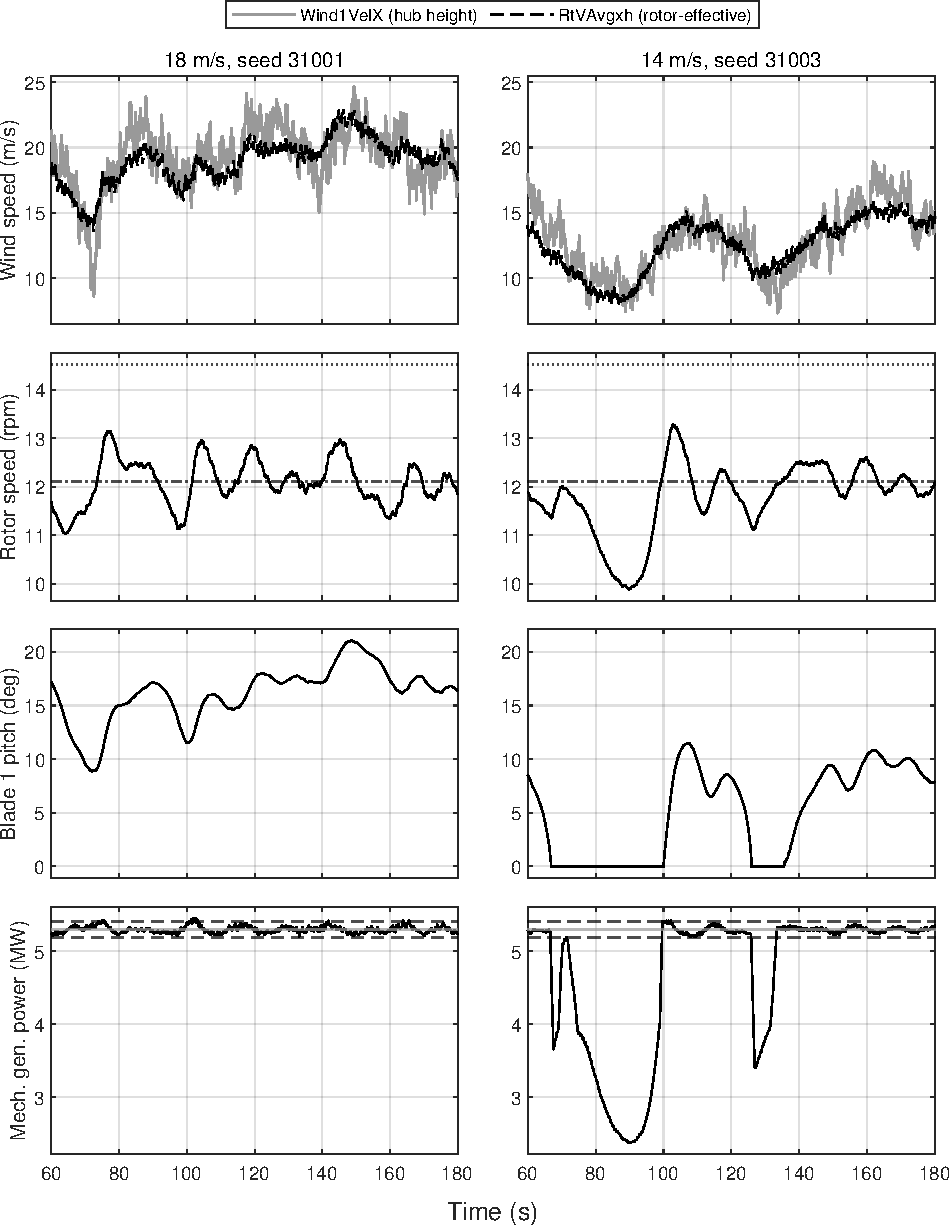
\includegraphics[width=\linewidth]{figures/E3_fig2_signals.pdf}
\caption{{\color{revQ1}Two runs of the qualification in above-rated wind, from 60 to 180~s: 18~m/s with seed 31001 (left) and 14~m/s with seed 31003 (right), the run that fails the power criterion. From top to bottom: wind speed at hub height (grey) and rotor-effective wind speed (dashed); rotor speed, with the rated rotor speed (dash-dotted) and 1.2 times this value (dotted, overspeed criterion); blade 1 pitch angle; mechanical generator power, with its rated value (grey) and $\pm 2$\,\% of it (dashed), the tolerance of the power criterion, which applies to the mean over a run and not to instantaneous values.}}
\label{fig:E3_signals}
\end{figure}
